\documentclass{article}
\usepackage[a4paper, margin=2.5cm]{geometry}
\usepackage[utf8]{inputenc}
\usepackage{graphicx}
\usepackage{url}
\usepackage{listings}
\usepackage{parcolumns}
\graphicspath{ {./images/} }
 
\title{Spectre \& Meltdown \\
\large{Speculative execution - performance hack or a massive vulnerability? \\ CS4028 Security: In-course assessment}}
\author{Konrad Dryja \\ 51552177 \\ k.dryja.15@abdn.ac.uk \\ University of Aberdeen}
\date{\today}
 
\begin{document}
 
\maketitle
 
\tableofcontents

\begin{abstract}
  As part of my CS4028 assessment, I would like to delve into the Spectre \& Meltdown vulnerabilities. I recognize that those are not offensive technology or tool per se, although both of them expose a major flaw which could easily be applied in one of them. I found researching this subject very interesting, as it taught me a lot about low-level CPU operations and how speculative execution can be used in nefarious ways. 
\end{abstract}
 
\section{Introduction}
 
The computing and security environments were shook in January 2018 when Google's Project Zero collaborating with security researchers discovered a major flaw in almost all consumer CPU. The hole allowed potentially a piece of code with no special privileges to read memory outside its own sandboxed environment (or even reading privileged parts of kernel memory). Day-to-day users perhaps wouldn't be impacted to a tremendous extent (it is claimed that until the flaw was discovered, no malicious use was detected [SOURCE]), but imagine running a production server in GCP, AWS or other major cloud provider - and having other malicious actors using Amazon being able to access your data from their own, virtualised containers. 

\begin{figure}[h]
\centering
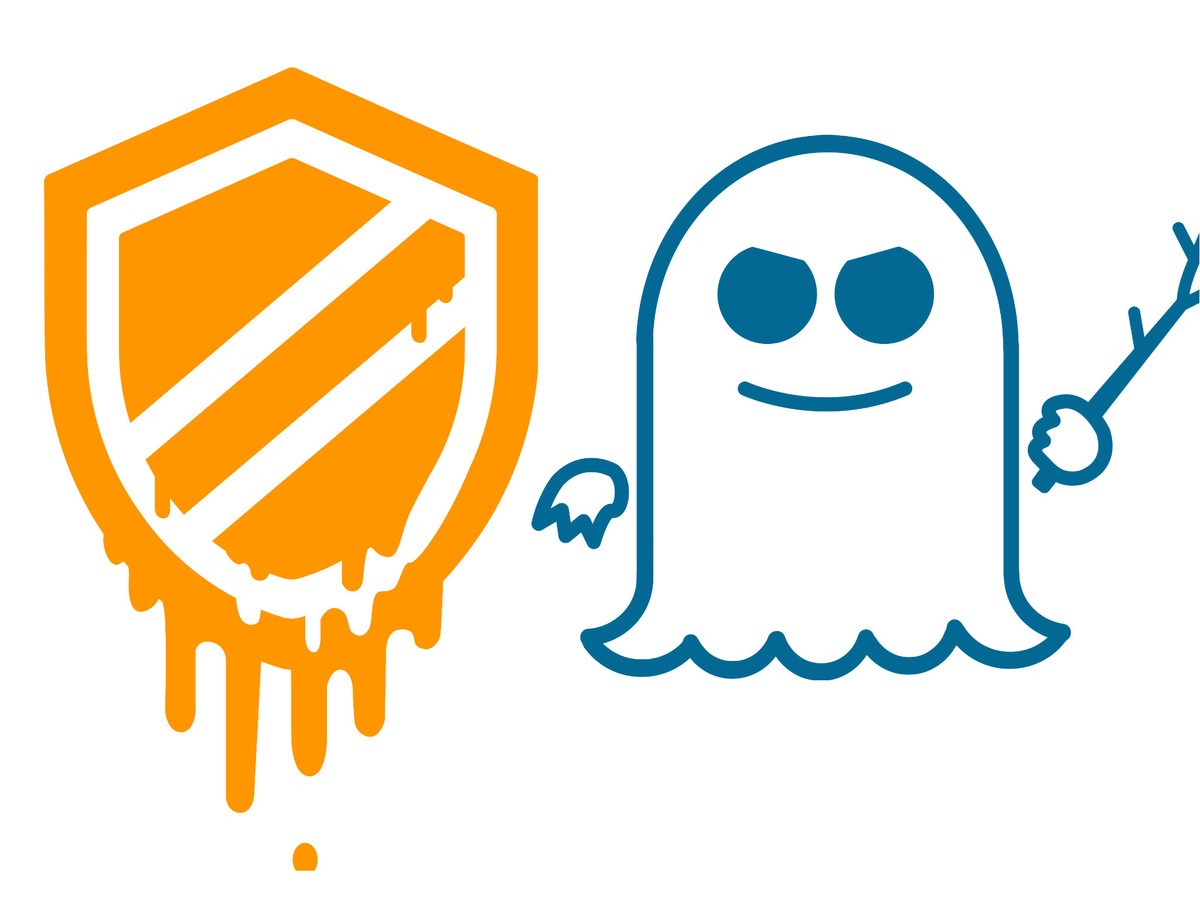
\includegraphics[width=0.3\textwidth]{logo}
  \caption{Graphic for Meltdown on the left, Spectre on the right.}
\end{figure}

As a word of introduction, the first discovery consisted of Spectre variant 1 \& 2, which was allocated Common Vulnerabilities and Exposures ID codes of CVE-2017-5753 [SOURCE] and CVE-2017-5715 [SOURCE] along with variant 3, which was dubbed Meltdown, with code CVE-2017-5754 [SOURCE].
 

\section{Background}

In order to understand how the vulnerabilities work, it is necessary to introduce some concepts and ideas that CPU manufacturers opted in for, also to overview low-level architecture of modern processors. In short, the biggest problems relate to Out of Order Execution (OOE), Branch Prediction (BP) and Branch Target Buffer (BTB) - all of those, in a way, were a mean to increase the performance of the chips and stand out on the market. At one point, Intel, AMD, ARM and more hit the ceiling with the clock speed, so they started seeking extra solutions - Branch Prediction was one of them. 

\paragraph{Branch Prediction}
To explain BP, I'm going to use an analogy one of the Stack Overflow users has introduced\cite{BranchpredictionSO}. The original poster discovered that simple array operation is significantly faster when the data is sorted, compared to unsorted - which at first seems like a compiler optimization, but eventually it was discovered that this artifact persists throughout different compilers or environments. 

\noindent\begin{minipage}{.45\textwidth}
\begin{lstlisting}[caption=Operation on an unsorted array,frame=tlrb]{Name}
from random import randint
arr = [randint(0,100) 
  for x in range(1000)]
# Start measuring time here
for y in range(1000000):
  for x in arr:
    if x > 50:
      print("more than 50")
\end{lstlisting}
\end{minipage}\hfill
\begin{minipage}{.45\textwidth}
\begin{lstlisting}[caption=Operation on a sorted array,frame=tlrb]{Name}
from random import randint
arr = [randint(0,100) 
  for x in range(1000)]
arr = sorted(arr)
# Start measuring time here
for y in range(1000000):
  for x in arr:
    if x > 50:
      print("more than 50")
\end{lstlisting}
\end{minipage}

Consider Listing 1 \& 2. Disregarding the time needed for sorting the array, seemingly the for-loop on Listing 2 was much faster. Finally, it was determined that it's not the compiler optimizing the machine code - but rather the CPU itself. Imagine CPU being a very heavy train, which takes a lot of time to get it started and lot of time to have it stopped. Our job, as an operator at the intersection, is to determine whether to flip the lever and change the direction of the tracks. Now assume that the past 50 trains took the route to the left and we have 51st train approaching. We can make educated guess and let the train preemptively go toward the left. Best case - we save a lot of time and train keeps going in the correct direction. Worst case, the train has to stop, roll back and go towards the right. Then we reflect on it and apply the finding during the future incidents.

Now, machine code is split into many branches - conditions. To increase performance, CPU will ``predict`` the outcome of the next operation, such that it'd be ready while a heavy operation (for example IO) is still pending.

\paragraph{Out of Order execution}
The technique is very similar to BP, in a way, as the ultimate goal is to speed up execution of instructions. It is a way to re-order and optimize the tasks to minimize the waiting time. I'd like to also point out the existence of \textbf{CPU cache}. Modern computers can store long-standing, persistent data on Solid State or spinning Drives, OS will often load and store running application within RAM. But access to either is going to be horribly slow, considering that modern CPUs run at clock speed of over 3GHz, which is 3000000000 clock cycles every second. To avoid the wait for data to arrive from external sources, cores often have built-in, small and incredibly fast memory called L1, L2 \& L3 cache.

Imagine a simple program consisting of the following steps:
\begin{enumerate}
  \item Load X
  \item Load Y, Z
  \item Sum X, Y, store it in K
  \item Sum Y, Z, store it in V
  \item Sum K, V
\end{enumerate}

Let's also assume that Y and Z are already present in the CPU cache, but X will need to be retrieved from RAM. For the sake of the example, the former operation takes 1 CPU cycle and the latter takes 3 (in reality though, the difference is much, much, much greater).

\begin{figure}[ht]
\centering
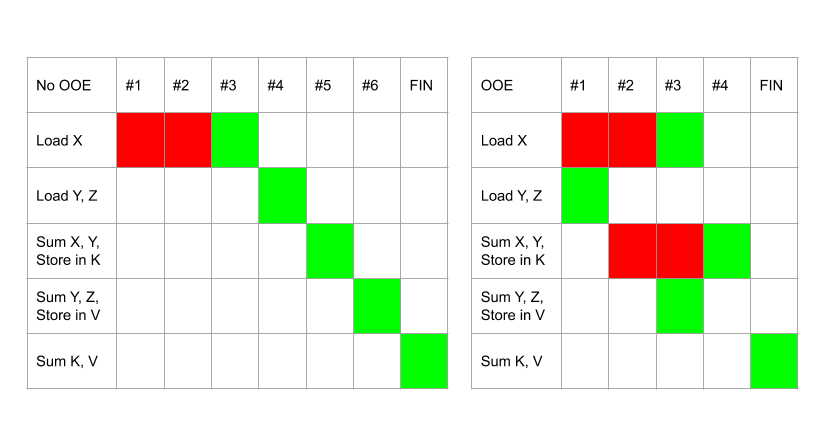
\includegraphics[width=0.9\textwidth]{OOE}
  \caption{OOE optimization}
\end{figure}

As per Figure 2, the execution would be halted at the first step, in order to retrieve the X from RAM, with the entire program taking 7 cycles. On the other hand, OOE optimizer would recognize the blocker and execute step 2, 4 BEFORE even reaching that point. That way, the entire operation can be closed only in 5 cycles.

% \addcontentsline{toc}{section}{Unnumbered Section}
% \section*{Unnumbered Section}
% lol 
 
\section{Meltdown \& Spectre}
 
Having covered the background behind the attack and feature it exploits, we can finally progress to the description itself. As mentioned at the beginning of the paper, it is necessary to distinct between Meltdown and Spectre, as ultimately they reach a different goal. Together, they are part of "branch target injection" class of vulnerabilities. The most impressive and scariest part is that in no way it exploits any of the software flaws, nor it is easy or even possible to patch it. Official recommendation by Intel is to completely replace the hardware with newer revisions with revised architecture no longer susceptible to those kind of attacks.

I'd like to present two different examples, as described in the original papers\cite{kocher2018spectre}\cite{lipp2018meltdown} released by Google's Project Zero. First would be an attack on Just-in-Time compiler of JavaScript. Which in theory means, that simply loading malicious website and executing the code would be enough to leak sensitive information from the computer itself.

The other would be a simple C program with the capability of reading privileged data, which otherwise would not be accessible and any attempts would result in either segmentation or page faults.

\paragraph{Meltdown}
Let's first though clear the disambiguation between the two. As we might know, kernel is utilizing its own page table, which should never be accessible by the user. This might hold information such as passwords, keyrings or other privileged information - important for running of the system (e.g. TLS connections). This would only be available when context switch happens into kernel model.

To increase the performance, modern CPU manufacturers map the kernel page-table space to every running process. This speeds up context switching and limits page faults. Of course, the address space is scrambled and protected by privileged bit meaning any access attempts will result in denials - and that's where speculative execution comes in action. Combination of Branch Prediction and Out of Order Execution gives the attacker the power to run any code at will with reasonable throughput.

\pagebreak
\begin{lstlisting}[caption=Speculative execution,frame=tlrb, numbers=left, firstnumber=1]{Name}
char testArray[256 * 64];

flush_cache(testArray);

char x = * kernelSpace; // Will cause segmentation fault
testArray[x * 64]++; // Will be executed speculatively

for(int i=0; i<256; i++)
{
  if(is_cached(testArray[i * 64])
  {
    // Cache hit! Found secret bit.
  }
}
\end{lstlisting}

In Listing 3, I have included a very high overview of the idea behind Meltdown. I will try to explain everything line-by-line before jumping into a real Proof-of-Concept working example.
\begin{enumerate}

  \item [1] Let's start with initiating our testArray - that's the entity that we're going to use to detect privileged information. We're planning to store 256 elements in it - and since L-cache is usually divided into rows 64-bits each, we multiply it by that number. 
  \item [3] We want to evict all current information residing in L-cache. This step highly depends on architecture and used compiler, usually it comes down to writing large quantities directly to CPU.
  \item [5] Normally, we'd be looking to wrap line 5 and 6 in a try-catch block, as in 5th line, we'd be attempting to access privileged information, causing segfault - so execution of the program would be dropped and all results discarded.
  \item [6] Assuming the information from previous step, the CPU tries to optimize the execution and PREDICTS that line 5 won't segfault, thus running the operation and saving the results in L-cache. But, once the clock actually reaches the forbidden operation, the results are discarded and rolled back, showing the fault. Though the results are still in cache...
  \item [8-14] This is the crucial and last step in the whole operation. We're simply iterating over all elements of our testArray and measuring the access time. is\_cached()'s job would be to tell us how long it takes to retrieve given bit from the array. As retrieval from L-cache is significantly faster, we can make an assumption that the operation was indeed speculatively executed and the secret bit was leaked... Repeat for the remaining of the array.

\end{enumerate}

Having explained the absolute basics behind the attack, let's try executing a real-life proof-of-concept showcasing the possibilities. 

\section{Mitigation}

\bibliographystyle{unsrt}
\bibliography{assessment}
 
\end{document}
